\documentclass{scrartcl}
\usepackage[utf8]{inputenc}
\usepackage[english]{babel}
\usepackage[T1]{fontenc}

\parindent 0pt
\parskip 0.5em

\title{Assignment 5}
\author{Jakob Wittmann\\Dominik Schmidt}
\date{\today}

\usepackage{hyperref}
\usepackage[all]{hypcap}
\hypersetup{pdfborder = {0 0 0}, colorlinks=true, allcolors=black, urlcolor=blue}
\usepackage[margin=2.5cm]{geometry}
\usepackage{booktabs}
\usepackage{array}
\setlength{\tabcolsep}{.3em}

\usepackage{float}
\usepackage[export]{adjustbox}
\usepackage{amsmath}
\usepackage{listings}
\lstset{basicstyle=\ttfamily,breaklines=true}
\def\dd{\mathrm{d}}
\def\ml{\mathrm{\frac{mmol}{h}}}

\usepackage{enumitem}
\setlist[enumerate]{label=\alph*), labelsep=*}

\begin{document}
\maketitle
\section{Form Polymer}
	\begin{enumerate}
		\item 
			\begin{align}
				\frac{\dd A}{\dd t} &= F1 - F2\\
				\frac{\dd B}{\dd t} &= F2 + F5 - F3 - F4\\
				\frac{\dd C}{\dd t} &= F3 - F_{obj} - F6\\
				\frac{\dd D}{\dd t} &= F4 - F5 - F7 - 2F_{obj} - F8\\
				\frac{\dd E}{\dd t} &= F6 + F7 - F_{obj}\\
			\end{align}
		\item $2.5 \mathrm{\frac{mmol}{h}}$
		\item 
			\begin{equation*}
				\begin{array}{r@{\;\leq\;}c@{\;\leq\;}l}
					10 \ml & F1 & 10 \ml \\
					10 \ml & F2 & 10 \ml \\
					0 \ml & F3 & 5 \ml\\
					0 \ml & F4 & \infty \ml\\
					0 \ml & F5 & \infty \ml\\
					0 \ml & F6 & 2.5 \ml\\
					0 \ml & F7 & 2.5 \ml\\
					0 \ml & F8 & 10 \ml\\
					0 \ml & F_{obj} & 2.5 \ml
				\end{array}
			\end{equation*}
		\item 
			\begin{equation*}
				\begin{array}{r@{\;\leq\;}c@{\;\leq\;}l}
					10 \ml & F1 & 10 \ml \\
					10 \ml & F2 & 10 \ml \\
					2.5 \ml & F3 & 5 \ml\\
					5 \ml & F4 & \infty \ml\\
					0 \ml & F5 & \infty \ml\\
					0 \ml & F6 & 2.5 \ml\\
					0 \ml & F7 & 2.5 \ml\\
					0 \ml & F8 & 0 \ml\\
					0 \ml & F_{obj} & 2.5 \ml
				\end{array}
			\end{equation*}
	\end{enumerate}
\section{2}
	\begin{enumerate}
		\item Assuming $V_4=0$
			\begin{align}
				V_{bio} &= x + \frac{1}{2} (1-x) \\
				V_{efni} &= \frac{1}{2} (1-x)\\
				x &= 2\cdot (V_{bio}-\frac{1}{2} = 2V_{bio} - 1\\
				V_{efni} &= \frac{1}{2} ( 1 - 2V_{bio} + 1) = 1-V_{bio}
			\end{align}
			\begin{figure}[H]
				\centering
				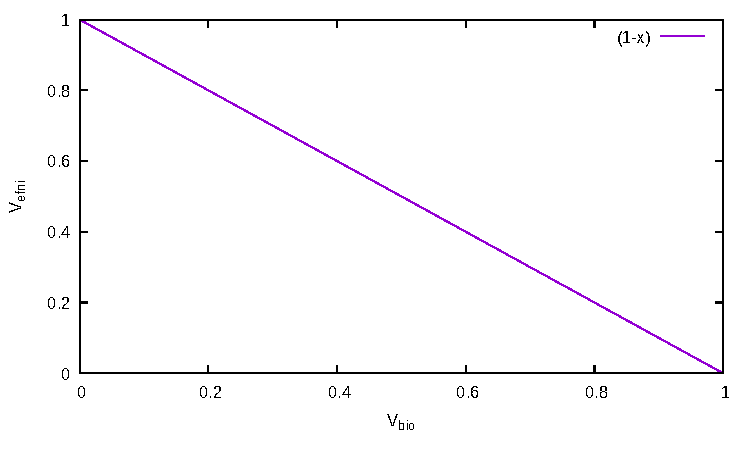
\includegraphics{2_a.pdf}
				\caption{Product vs. biomass-production in the original organism}
			\end{figure}
		\item If $V_1$ and $V_4$ are removed, the organism is forced to take the path $(V_2,V_3,\{V_{bio},V_{efni}\})$ 
			\begin{align}
				V_{bio} &= \frac{1}{2}\\
				V_{efni} &= \frac{1}{2}\\
				V_{efni} &= V_{bio}
			\end{align}
			\begin{figure}[H]
				\centering
				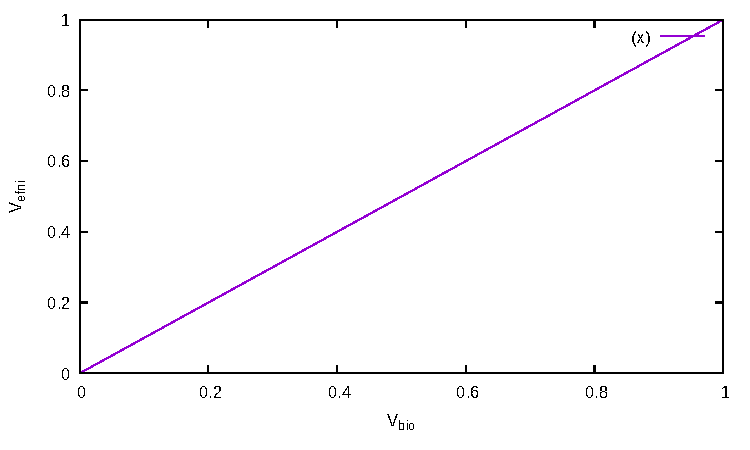
\includegraphics{2_b.pdf}
				\caption{Product vs. Biomass-production in the mutant}
			\end{figure}
		\item If there is enough nutrition in the environment, the organism will optimize its metabolism to grow. If we want to nudge it to produce our target compound, it will be forced to do so. 
			Furthermore, if we want to have exponentially growing production of our compound, it is beneficial to couple production an growth together
	\end{enumerate}
\section{Python}
    \lstinputlisting{Program/output.txt}
	\subsection{Graphs}
		\begin{figure}[H]
			\centering
			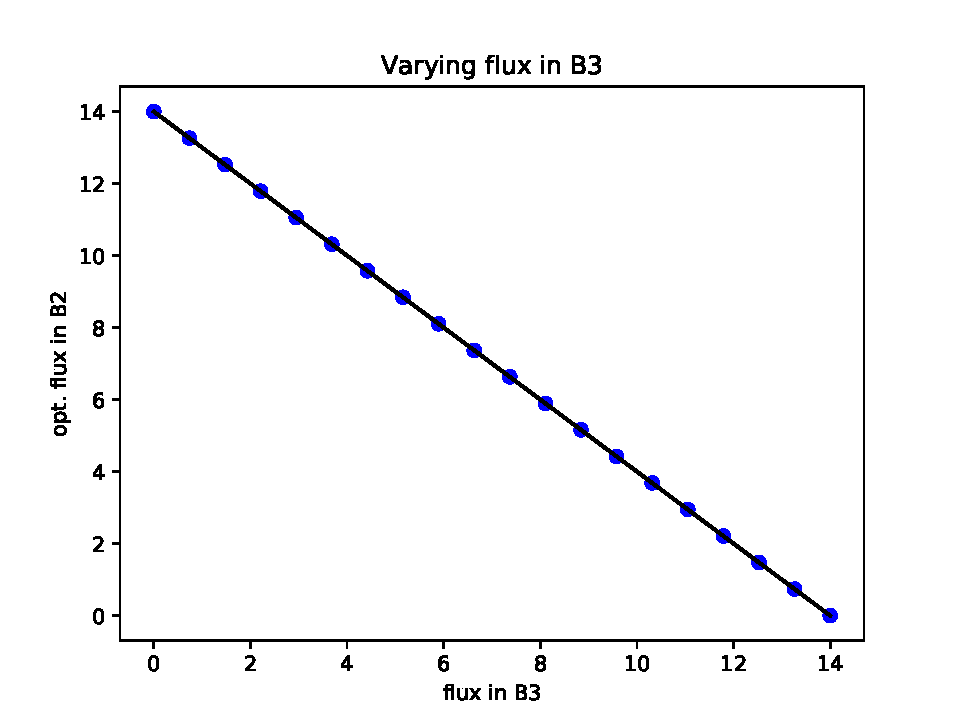
\includegraphics[max width=0.8\linewidth]{Program/Figure_1.pdf}
			\caption{Graph for question d)}
		\end{figure}
		\begin{figure}[H]
			\centering
	     		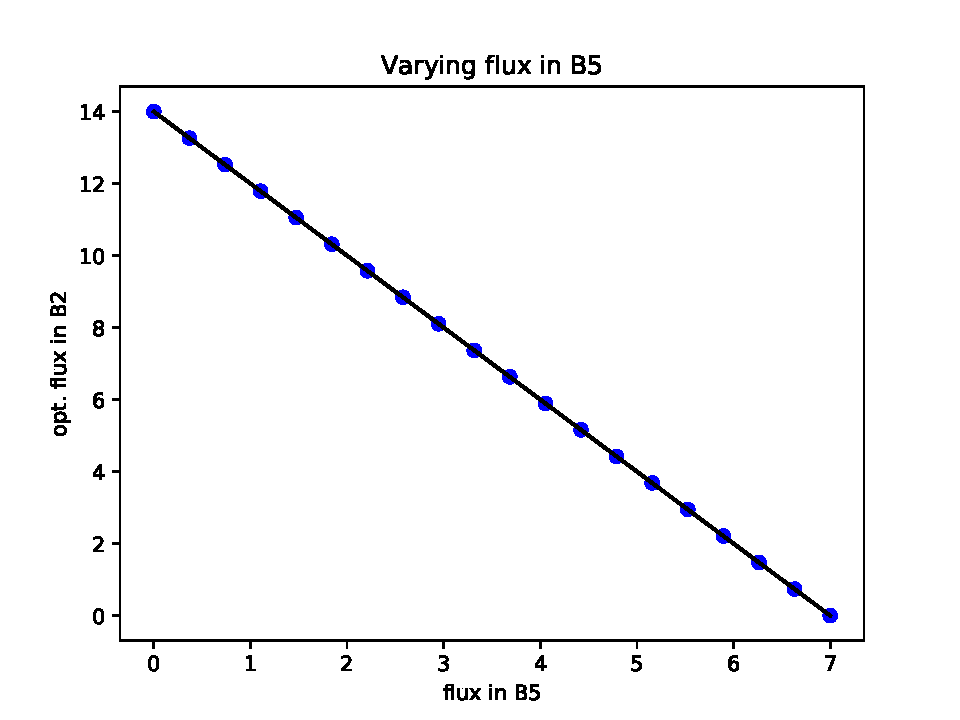
\includegraphics[max width=0.8\linewidth]{Program/Figure_2.pdf}
			\caption{Graph for question g)}
		\end{figure}
\end{document}
